\begin{figure}[t]
\begin{tabular}{ccc}
\begin{subfigure}[b]{0.32\textwidth}
\begin{center}
{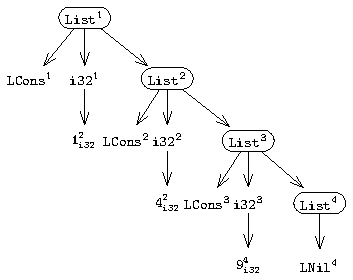
\includegraphics[scale=0.8]{chapters/figures/figParseTreeList3.pdf}}
\end{center}
\caption{\label{fig:listParseTree}{\small\tt List = LNil | \newline LCons(i32, List)}}
\end{subfigure}%
&
\begin{subfigure}[b]{0.22\textwidth}
\begin{center}
{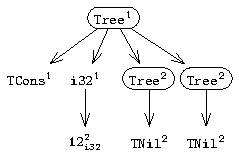
\includegraphics[scale=0.78]{chapters/figures/figParseTreeTree2.pdf}}
\vspace{10px}
\end{center}
\caption{\label{fig:treeParseTree}{\footnotesize\tt Tree = TNil | \newline TCons(i32, Tree, Tree)}}
\end{subfigure}%
&
\begin{subfigure}[b]{0.4\textwidth}
\begin{center}
{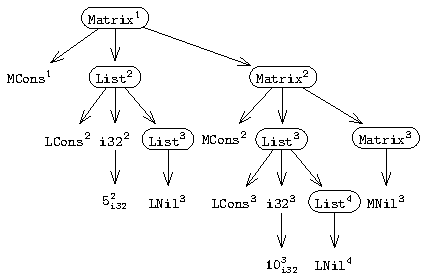
\includegraphics[scale=0.78]{chapters/figures/figParseTreeMatrix2.pdf}}
\end{center}
\caption{\label{fig:matrixParseTree}{\tt Matrix = MNil | \newline MCons(List, Matrix)}}
\end{subfigure}%
\\
\end{tabular}
\vspace{-12px}
\caption{\label{fig:parseTrees}Parse Trees with Depths (shown as superscript) for {\tt List}, {\tt Tree}, and {\tt Matrix2D}}
\end{figure}
